\documentclass[10pt,letterpaper]{article}
\usepackage{hyperref}
\usepackage{graphicx}
\usepackage{geometry}
\usepackage{amsmath}

\begin{document}

\title{A biology-inspired neural network evolving through natural selection}
\author{Souvik Das}
\maketitle

\begin{abstract}
We describe a biology-inspired time-stepped simulation of a neural network that structures itself by competing against mutated copies of itself. The simulated neurons seek to capture the functional essence of a biological neuron as a function of time. We find a condition between the inputs to the neuron and its activation potential that needs to be met for the neuron to fire continuously, and conjecture that a similar condition may also exist in biology. The neural network encodes synaptic chemical concentrations between neurons that changes over the course of a network's lifetime based on simple rules of reinforcement and decay. The network also encodes the physical distance or connectivity between neurons that evolves over generations through natural selection. Multiple copies of these neural networks are instantiated in a game world, each with small random mutations in the connectivities.



\end{abstract}
\clearpage

\tableofcontents
\clearpage

\section{The simulated neuron}

The simulated neuron used in this system tries to capture, through a time-stepped simulation, the functional essence of a biological neuron. A neuron receives input potentials $q_i$ (between -1 and 1) from the output of several other neurons, over time. The neuron sums up these potentials, at every time-step, and if the sum exceeds a threshold $Q_{th}$ it fires an activation potential that is then communicated via synapses to other neurons. After firing, the neuron's own potential drops to a small value below the baseline of 0 and then decays back to 0 by a factor of $k_p$ at every time-step. This decay constant for the potential, $k_p$, is always applied on the neuron and causes the potential to decay back to 0 even if the threshold has not been met and the neuron not been fired. Fig.~\ref{fig:c_potential_time} shows the potential of a single neuron that has been fired (red) and one that has not been fired (blue).

\begin{figure}[thp]
\centering
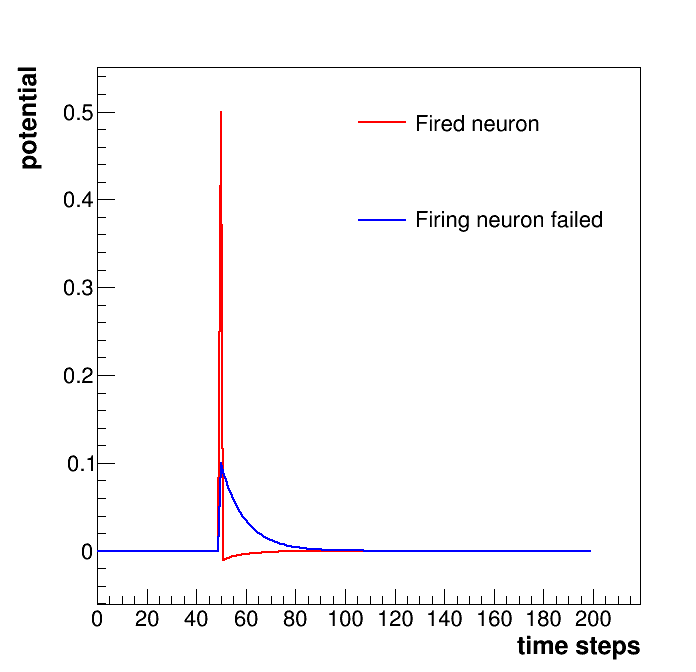
\includegraphics[width=0.6\textwidth]{c_potential_time.png}
\caption{The potential of a single neuron is plotted as a function of time. The red curve is for a neuron that is stimulated with a potential greater than the threshold $Q_{th}$ = 0.4 at time 50. It fires on its output and then drops its potential to -0.01. Thereafter, the potential decays by a factor of $k_p$ = 0.9 every time-step back to 0. In blue is the same neuron stimulated with a potential less than $Q_{th}$. It does not fire and the potential simply decays by $k_p$ back to 0.}
\label{fig:c_potential_time}
\end{figure}

\subsection{Output frequency from input frequency}

We can derive the frequency at which the neuron will fire if it is stimulated with a potential of $q$ applied every $t$ time-steps, i.e. with a frequency of $f_{in} = 1/t$. Since the potential will decay by a factor of $k_p$ at every time-step, the potential will reach $Q_{th}$ after $n$ time steps where:

\begin{equation*}
q(1 + k_p^t + k_p^{2t} ... + k_p^{nt}) = Q_{th}
\end{equation*}  

This is the sum of a geometric series, and we can write it in closed form as Eq.~\ref{eq:neuron:eq1}.

\begin{equation}
\label{eq:neuron:eq1}
\frac{Q_{th}}{q} = \frac{1-k^{t(n+1)}}{1-k^t}
\end{equation}

This can be solved for $n$ to derive the output frequency of the neuron $f_{out} = 1/nt$. The solution for $n$ is written in Eq.~\ref{eq:neuron:n}.

\begin{equation}
\label{eq:neuron:n}
n = \frac{\log(1-\frac{Q_{th}}{q}(1-k^t))}{t\log(k)}-1
\end{equation}

For this to be true, i.e. for the total potential to ever reach $Q_{th}$, the argument of the logarithm in the numerator has to be positive. This implies a minimum frequency of input firing given by Eq.~\ref{eq:neuron:fin}. If this condition is not met, the neuron does not reach the firing threshold as shown by the blue curve in Fig.~\ref{fig:c_potential_time_sawtooth}a. When the condition is met, the neuron repeatedly fires in intervals of $nt$ given by Eq.~\ref{eq:neuron:n} as shown by the red curve in Fig.~\ref{fig:c_potential_time_sawtooth}b. \textit{We conjecture that such a condition may also exist for the firing of biological neurons.}

\begin{equation}
\label{eq:neuron:fin}
\frac{1}{f_{in}} = t < \frac{\log(1-q/Q_{th})}{\log(k)}
\end{equation}

\begin{figure}[thp]
\centering
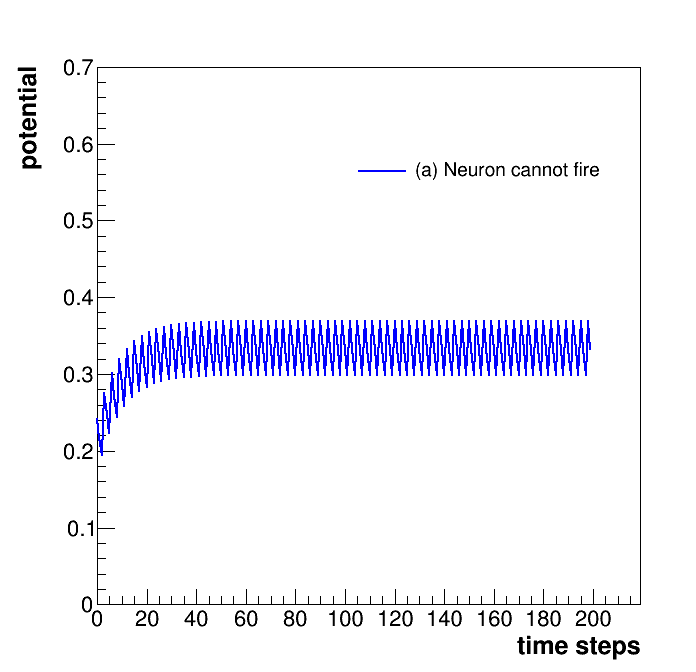
\includegraphics[width=0.49\textwidth]{c_potential_time_sawtooth_a.png}
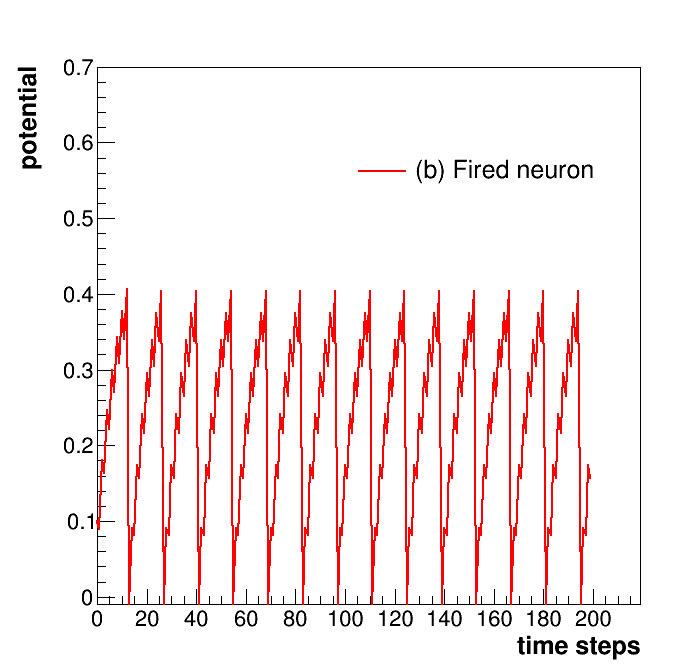
\includegraphics[width=0.49\textwidth]{c_potential_time_sawtooth_b.png}
\caption{(a) LEFT. The neuron is programmed with a potential threshold $Q_{th}$ = 0.4, and a potential decay constant $k_p$ = 0.90. It is stimulated with potentials of $q$ = 0.1 applied every $t$ = 3 timesteps. According to Eq.~\ref{eq:neuron:fin}, $t$ needs to be less than 2.7 for the neuron to fire and therefore the neuron does not fire. (b) RIGHT. The neuron is now stimulated with $q$ = 0.1 applied every $t$ = 2 timesteps, and therefore it fires.}
\label{fig:c_potential_time_sawtooth}
\end{figure}

... \textit{Show the relationship between output and input frequencies. Connection with sigmoid.}

\subsection{Synaptic weights}

Neurons are connected to each other through synapses. We simulate the synaptic weight $w$ that corresponds to the concentration of a generic neurotransmitter in the synapse in time-steps as well. The value of the weight, $w$, lies between 0 and 1. If the output of neuron $i$ feeds into an input of neuron $j$, the synaptic weight is denoted by $w_{ij}$. When neuron $i$ fires, a fraction of the action potential $w_{ij}/\sum_{k}w_{ik}$ is transmitted to neuron $j$. $k$ is an index that runs over all the other neurons that neuron $i$ feeds into.

The weight of a synapse is reinforced every time a signal passes through it. The reinforcement is implemented as an increase of the weight $w$ by $\alpha(1-w)$. This is a form of Hebbian learning that implements unsupervised learning in the neural network. The weight also decays by a factor of $\beta$ at every time-step.




\section{The brain}

\subsection{Neural connections}

\subsection{Summary of mutation parameters}


\section{The natural selection environment}


\section{Learning to survive over generations}


\section{Punctuated equilibria}



\end{document} 

